\documentclass{article}

\usepackage[dblblindworkshop]{neurips_2026}

\workshoptitle{Foundation Models for Temporal Systems (FMTS)}

\usepackage[utf8]{inputenc}
\usepackage[T1]{fontenc}
\usepackage{hyperref}
\usepackage{url}
\usepackage{booktabs}
\usepackage{amsfonts}
\usepackage{amsmath}
\usepackage{nicefrac}
\usepackage{microtype}
\usepackage{xcolor}
\usepackage{graphicx}
\usepackage{float}
\usepackage{subcaption}

\title{Is the Reconstruction--Forecasting Tradeoff a Frontier\\or an Operating Point?}

\author{Arpit Goel\\ TwinSim Labs \\ arpit@thebrownkid.in}

\begin{document}

\maketitle

\begin{abstract}
Latent dynamical models for time series encode observations into a latent space
that must simultaneously support accurate reconstruction and accurate
forecasting.  When a single latent serves both roles, improving one objective
often degrades the other, creating an apparent Pareto frontier that practitioners
navigate by tuning a loss weight or choosing a latent dimension.  We argue that
this tradeoff is an artifact of architectural coupling, not a fundamental limit.
We propose a \emph{residual decoupling} architecture that separates the two
tasks across two latent spaces: a wide carrier trained purely for reconstruction,
and a narrow residual code derived from the carrier's temporal differences,
trained purely for forecasting via Dynamic Mode Decomposition (DMD).  Because the
two objectives share no trainable parameters after the teacher autoencoder is
frozen, reconstruction quality is preserved by construction.  On four dynamical
systems spanning linear, oscillatory, and spatiotemporal dynamics, the decoupled
model strictly Pareto-dominates the coupled baseline, improving both reconstruction
and forecast accuracy on every system; an ablation confirms that GRU-gated
accumulation is essential for stable rollouts.
\end{abstract}


\section{Introduction}

Autoencoder-based latent dynamical models encode a time series into a
low-dimensional latent space, apply a dynamics model in that space, and decode
back to observations.  The latent must serve two masters: the decoder needs an
encoding that preserves enough information to reconstruct $x_t$ faithfully,
while the dynamics model needs an encoding whose temporal evolution is
predictable.  These two demands are in tension.

The standard recipe trains on a weighted loss
$\mathcal{L} = (1-\alpha)\,\mathcal{L}_{\mathrm{rec}} + \alpha\,\mathcal{L}_{\mathrm{fcst}}$
and tunes $\alpha$ per
dataset~\citep{lusch2018deep,takeishi2017learning,otto2019linearly}.
Within the Koopman operator
framework~\citep{brunton2022modern,bevanda2021koopman}, deep autoencoders
learn latent coordinates where dynamics are
linear~\citep{yeung2019learning,champion2019data,gin2021deep};
locally-linear latent dynamics have also been explored for
control~\citep{watter2015embed}.
Physics-informed~\citep{erichson2019} and
consistent~\citep{azencot2020} variants add stability or consistency
penalties, but the fundamental design remains: one encoder, one latent, two
objectives.  The resulting tradeoff is widely
observed~\citep{cai2023hyvae,sener2018multi}.

We make a simple observation: if a teacher autoencoder already reconstructs
well, its carrier representation contains enough information about the dynamics
for a second model to derive a \emph{separate} encoding optimised purely for
forecasting.  No gradient from the forecasting objective ever needs to reach the
reconstruction pathway, so the tradeoff disappears by construction.
We demonstrate this on four dynamical systems: a residual decoupling architecture
consistently improves both reconstruction and forecasting
compared to the standard AE+DMD baseline.


\section{The Tradeoff}

Consider a Koopman-style autoencoder with latent dimension $k$ and a learned
linear transition $A$, trained on
$\mathcal{L} = (1{-}\phi)\,\mathcal{L}_{\mathrm{rec}} +
\phi\,\mathcal{L}_{\mathrm{lin}}$,
where $\mathcal{L}_{\mathrm{lin}} = \|E(x_{t+1}) - A\,E(x_t)\|^2$.
At $\phi{=}0$ the encoder optimises purely for reconstruction; at $\phi{=}1$
purely for linear predictability.  Sweeping $\phi$ traces out the Pareto
frontier of what a \emph{single coupled latent} can achieve.

Figure~\ref{fig:frontier} shows this frontier on three representative systems.
Reconstruction RMSE improves as $\phi \to 0$ and forecast RMSE improves as
$\phi \to 1$, but no single $\phi$ minimises both; the two objectives
genuinely compete for the same $k$ dimensions.  The frontier represents the
best the coupled architecture can do at any weight.

Our method decouples the two: a wide carrier $j \gg k$ serves reconstruction,
while a separate residual code of dimension $k$ serves forecasting.  Because
they share no parameters after phase~1, each objective is free to use its own
capacity fully.  On all systems the decoupled model sits
\emph{inside} the coupled frontier, achieving reconstruction near the $\phi{=}0$
extreme and forecast quality that the coupled model can only reach by
sacrificing reconstruction.

\begin{figure}[t]
\centering
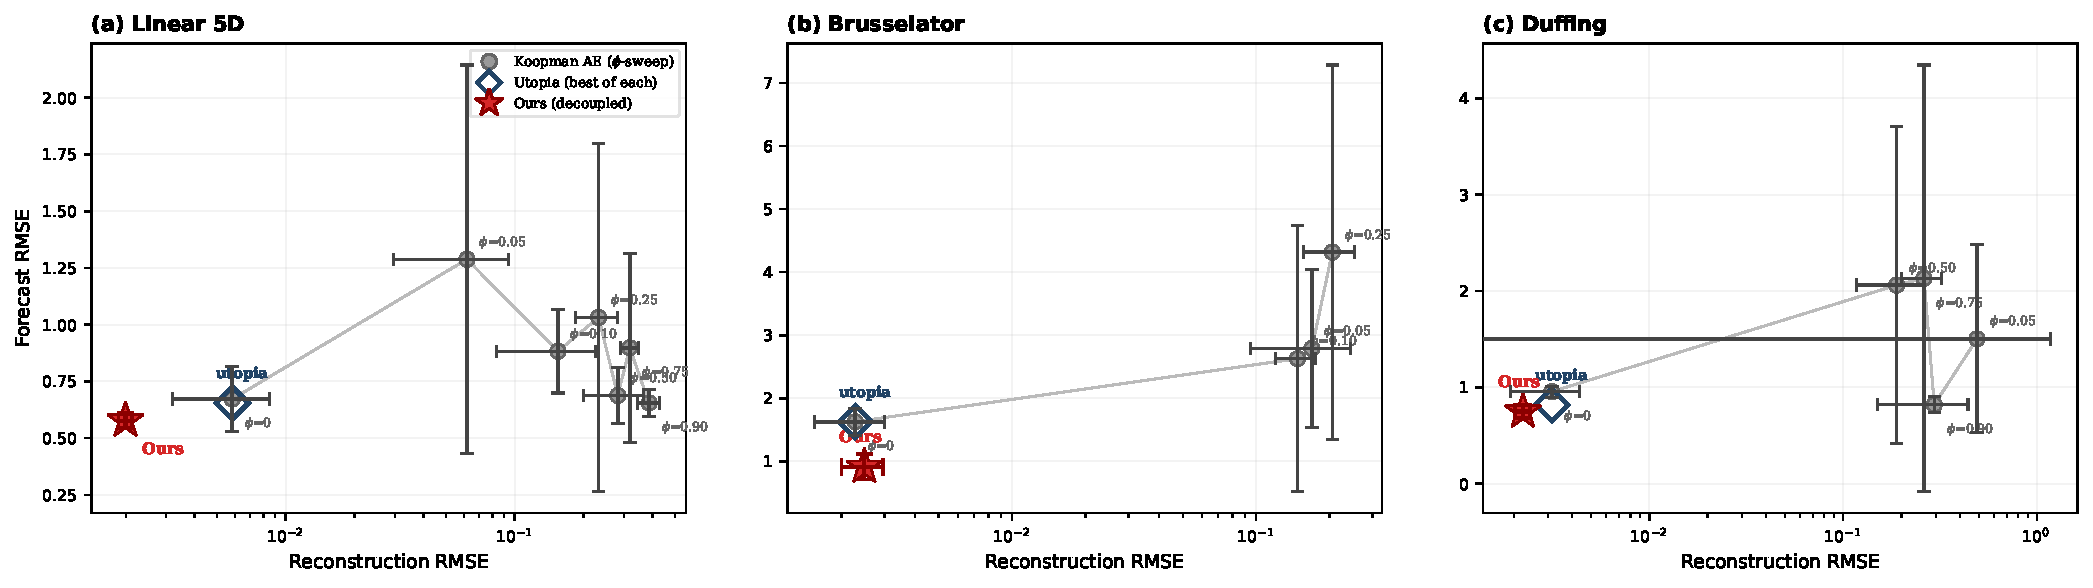
\includegraphics[width=\textwidth]{phi_sweep.png}
\caption{$\phi$-sweep for a Koopman AE (grey circles, connected; error bars
over 5 seeds): the Pareto frontier of a single coupled latent.  Our decoupled
model (\textcolor{red}{$\star$}) operates inside this frontier on all three
systems, achieving near-$\phi{=}0$ reconstruction with near-$\phi{=}1$
forecast quality.  The \textcolor{blue!60!black}{$\diamond$} marks the utopia
point (best recon, best forecast from the sweep); the gap between our star and
the utopia is the remaining room for architectural improvement.}
\label{fig:frontier}
\end{figure}


\section{Method}
\label{sec:method}

Our architecture decouples reconstruction from forecasting by introducing a
second latent space derived from the first.

\paragraph{Teacher autoencoder.}
An encoder $E: \mathbb{R}^n \to \mathbb{R}^j$ and decoder
$D: \mathbb{R}^j \to \mathbb{R}^n$ are trained as a standard
autoencoder~\citep{hinton2006reducing}.
The carrier $C_t = E(x_t) \in \mathbb{R}^j$ serves reconstruction:
$\hat{x}_t = D(C_t)$.  We choose $j$ large enough for near-perfect
reconstruction.

\paragraph{Residual compressor.}
With the teacher frozen, we compute carrier residuals
$\Delta C_t = C_{t+1} - C_t$ and train a compressor $f: \mathbb{R}^j \to
\mathbb{R}^k$ and decompressor $m: \mathbb{R}^k \to \mathbb{R}^j$ as a
second autoencoder on $\Delta C$:
\begin{equation}
  \mathcal{L}_{\mathrm{resid}} = \left\| \Delta C_t - m(f(\Delta C_t)) \right\|^2.
  \label{eq:resid}
\end{equation}
The residual code $b_t = f(\Delta C_t) \in \mathbb{R}^k$ with $k \ll j$
captures the temporal dynamics in a compressed form, analogous to residual
learning~\citep{he2016deep}, amenable to linear prediction.

\paragraph{GRU-gated accumulation.}
During forecasting, the carrier evolves by accumulating decoded residuals.
Naively adding $C_{t+1} = C_t + m(b_t)$ compounds small errors.
We replace the addition with a GRU cell~\citep{cho2014learning}:
\begin{equation}
  C_{t+1} = \mathrm{GRU}\!\bigl(m(b_t),\; C_t\bigr),
  \label{eq:gru}
\end{equation}
trained (with $E$, $D$, $f$, $m$ frozen) to predict the true next carrier.

\paragraph{Post-hoc DMD.}
With all neural components frozen, we fit a DMD~\citep{schmid2010dmd} matrix
$A \in \mathbb{R}^{k \times k}$ on the training residual codes:
$A = B_{1:}^\top (B_{:-1}^\top)^\dagger$, where $B$ is the matrix of
$b_t$ vectors.  Forecasting proceeds as
$b_{T+\tau} = A^\tau b_T$, decoded through $m$ and accumulated through the GRU
into the carrier, then decoded through $D$ to observations.

\paragraph{Three-phase training.}
The schedule is:
\textbf{Phase~1:} train $E + D$ (reconstruction).
\textbf{Phase~2:} freeze $E + D$; train $f + m$ on carrier residuals, then train
the GRU on $(m(f(\Delta C)), C_t) \to C_{t+1}$.
\textbf{Post-hoc:} fit DMD on frozen $b$ trajectory.
By construction, no forecast gradient ever reaches $E$ or $D$, so
reconstruction quality is preserved exactly.

\paragraph{Fairness constraint.}
Both the baseline AE and our model use DMD as the sole forecast head, and both
forecast in $\mathbb{R}^k$.  The baseline uses $k$ for everything; ours adds a
wider carrier $j > k$ for reconstruction only.  All models are trained until
loss convergence (400 epochs per phase, verified to plateau).


\section{Experiments}

\paragraph{Setup.}
We evaluate on four smooth dynamical systems: a linear 5D system with two
frequencies, the Brusselator chemical oscillator, the forced Duffing
oscillator, and Lorenz-96 (20D spatiotemporal).
Two-dimensional systems are delay-embedded with 5 delays to produce 10D
observations; higher-dimensional systems use their native state.  We set
carrier $j=8$ for systems up to 10D and $j=12$ for Lorenz-96; residual
dimension $k$ matches the baseline AE dimension.
All models share the same architecture width ($h=64$), training epochs
(400 per phase), batch size (512), and are run over 5 random seeds; we report
mean $\pm$ standard deviation.

\paragraph{Metrics.}
Reconstruction RMSE on held-out test data.  Forecast RMSE on 500-step
rollouts initialised from the first test point.  Both are computed in physical
(un-normalised) coordinates.

\paragraph{Pareto dominance.}
Method A \emph{Pareto-dominates} method B if A achieves reconstruction and
forecast RMSE each no worse than B, with at least one strictly lower.


\newcommand{\tpm}[2]{$#1${\tiny$\pm$\!$#2$}}
\begin{table}[t]
\caption{Results on four dynamical systems (mean$\pm$std over 5 seeds).
\textbf{Bold} marks where Ours improves over AE+DMD.
Resid+add ablates the GRU gate (naive carrier addition).}
\label{tab:main}
\centering
\small
\setlength{\tabcolsep}{3pt}
\begin{tabular}{lcc cc cc cc}
\toprule
& & & \multicolumn{2}{c}{AE+DMD} & \multicolumn{2}{c}{Resid+add} & \multicolumn{2}{c}{Ours (Resid+GRU)} \\
\cmidrule(lr){4-5} \cmidrule(lr){6-7} \cmidrule(lr){8-9}
System & obs & $k$ & Recon & Fcst & Recon & Fcst & Recon & Fcst \\
\midrule
Linear 5D     & 5D  & 4
  & \tpm{.005}{.002} & \tpm{.67}{.14}
  & \tpm{.002}{.000} & \tpm{6.0}{2.3}
  & \textbf{\tpm{.002}{.000}} & \textbf{\tpm{.58}{.03}} \\
Brusselator   & 10D & 3
  & \tpm{.002}{.001} & \tpm{1.66}{.26}
  & \tpm{.002}{.001} & \tpm{3.4}{2.6}
  & \tpm{.002}{.000} & \textbf{\tpm{.92}{.20}} \\
Duffing       & 10D & 3
  & \tpm{.003}{.001} & \tpm{.95}{.06}
  & \tpm{.002}{.000} & \tpm{2.1}{1.1}
  & \textbf{\tpm{.002}{.000}} & \textbf{\tpm{.75}{.07}} \\
Lorenz-96     & 20D & 10
  & \tpm{1.76}{.03} & \tpm{4.73}{.16}
  & \tpm{1.40}{.02} & \tpm{100}{15}
  & \textbf{\tpm{1.41}{.03}} & \textbf{\tpm{4.47}{.08}} \\
\bottomrule
\end{tabular}
\end{table}


\paragraph{Main results.}
Table~\ref{tab:main} reports all four systems.  On every system the decoupled
model Pareto-dominates the coupled baseline: reconstruction improves or matches
while forecast accuracy also improves.
On Linear~5D, reconstruction drops from $0.005$ to $0.002$ ($2.5\times$) while
forecast improves from $0.67$ to $0.58$.  On Brusselator, reconstruction is
matched within noise while forecast improves $1.8\times$ ($1.66 \to 0.92$).
On Duffing, both metrics improve ($0.95 \to 0.75$ forecast, $0.003 \to 0.002$
reconstruction).  On the 20D Lorenz-96 system, reconstruction improves
$1.25\times$ and forecast improves $1.06\times$, demonstrating that the
decoupling extends to higher-dimensional spatiotemporal dynamics.

\paragraph{Ablation: GRU gate.}
The Resid+add column ablates the GRU gate, accumulating carriers via naive
addition $C_{t+1} = C_t + m(b_t)$.  Decoupling alone preserves reconstruction
quality, but without the GRU gate forecast errors compound over the 500-step
rollout: Resid+add forecast RMSE exceeds AE+DMD on every system, by
$2{-}9\times$ on the oscillatory benchmarks and diverging to RMSE $100$ on
Lorenz-96.  The GRU gate (Eq.~\ref{eq:gru}) is essential for stable rollouts.

\section{Discussion and Conclusion}

The reconstruction--forecasting tradeoff arises wherever a single latent space
must serve both objectives: Koopman autoencoders~\citep{lusch2018deep,otto2019linearly},
latent ODE models~\citep{chen2018neural,rubanova2019latent}, and hybrid
VAEs~\citep{cai2023hyvae} all face it.  Our decoupling principle, separating the
representation that the decoder reads from the one that the dynamics model
predicts, is not specific to the DMD forecast head or the systems tested here;
it applies to any latent dynamical model whose encoder is shared between
reconstruction and prediction.

The $\phi$-sweep frontier (Figure~\ref{fig:frontier}) represents the best a
coupled latent can achieve at any weighting.  Our decoupled model operates
inside this frontier, but does not reach its corners simultaneously.  The gap
between our operating point and the \emph{utopia point} (best-of-sweep
reconstruction paired with best-of-sweep forecast) measures how much room
remains for architectural improvement.

Using DMD as the sole forecast head for both methods isolates the architectural
contribution from the dynamics model.  The results are lower bounds on what a
nonlinear forecast head could achieve in this framework.

\paragraph{Limitations.}
The benchmark is limited to smooth, deterministic ODEs; real-world noise,
nonstationarity, and high dimensionality may change the balance.  The
architecture adds parameters ($f$, $m$, GRU) beyond the baseline AE, and we do
not tune hyperparameters per system beyond setting $j$ and $k$ by observation
dimension.

\paragraph{Takeaway.}
The tradeoff is not a Pareto frontier; it is an operating point imposed by
asking one latent to do two jobs.  Decoupling the two across separate latent
spaces consistently improves both reconstruction and forecast quality, and the
$\phi$-sweep frontier shows how much further a future architecture might go.

\bibliographystyle{plainnat}
\begin{thebibliography}{99}

\bibitem[Azencot et al.(2020)]{azencot2020}
O.~Azencot, N.~B. Erichson, V.~Lin, and M.~W. Mahoney.
\newblock Forecasting sequential data using consistent Koopman autoencoders.
\newblock In \emph{ICML}, pages 475--485, 2020.

\bibitem[Bevanda et al.(2021)]{bevanda2021koopman}
P.~Bevanda, S.~Sosnowski, and S.~Hirche.
\newblock Koopman operator dynamical models: Learning, analysis and control.
\newblock \emph{Annual Reviews in Control}, 52:197--212, 2021.

\bibitem[Brunton et al.(2022)]{brunton2022modern}
S.~L. Brunton, M.~Budi\v{s}i\'{c}, E.~Kaiser, and J.~N. Kutz.
\newblock Modern {K}oopman theory for dynamical systems.
\newblock \emph{SIAM Review}, 64(2):229--340, 2022.

\bibitem[Cai et al.(2023)]{cai2023hyvae}
B.~Cai, S.~Yang, L.~Gao, and Y.~Xiang.
\newblock Hybrid variational autoencoder for time series forecasting.
\newblock \emph{Knowledge-Based Systems}, 281:111079, 2023.

\bibitem[Champion et al.(2019)]{champion2019data}
K.~Champion, B.~Lusch, J.~N. Kutz, and S.~L. Brunton.
\newblock Data-driven discovery of coordinates and governing equations.
\newblock \emph{Proc.\ Natl.\ Acad.\ Sci.}, 116(45):22445--22451, 2019.

\bibitem[Chen et al.(2018)]{chen2018neural}
R.~T.~Q. Chen, Y.~Rubanova, J.~Bettencourt, and D.~Duvenaud.
\newblock Neural ordinary differential equations.
\newblock In \emph{NeurIPS}, 2018.

\bibitem[Cho et al.(2014)]{cho2014learning}
K.~Cho, B.~van Merri\"{e}nboer, C.~Gulcehre, D.~Bahdanau, F.~Bougares,
  H.~Schwenk, and Y.~Bengio.
\newblock Learning phrase representations using {RNN} encoder--decoder for
  statistical machine translation.
\newblock In \emph{EMNLP}, pages 1724--1734, 2014.

\bibitem[Erichson et al.(2019)]{erichson2019}
N.~B. Erichson, M.~Muehlebach, and M.~W. Mahoney.
\newblock Physics-informed autoencoders for Lyapunov-stable fluid flow
  prediction.
\newblock \emph{arXiv preprint arXiv:1905.10866}, 2019.

\bibitem[Gin et al.(2021)]{gin2021deep}
C.~Gin, B.~Lusch, S.~L. Brunton, and J.~N. Kutz.
\newblock Deep learning models for global coordinate transformations that
  linearize {PDE}s.
\newblock \emph{European J.\ Appl.\ Math.}, 32(3):515--539, 2021.

\bibitem[He et al.(2016)]{he2016deep}
K.~He, X.~Zhang, S.~Ren, and J.~Sun.
\newblock Deep residual learning for image recognition.
\newblock In \emph{CVPR}, pages 770--778, 2016.

\bibitem[Hinton and Salakhutdinov(2006)]{hinton2006reducing}
G.~E. Hinton and R.~R. Salakhutdinov.
\newblock Reducing the dimensionality of data with neural networks.
\newblock \emph{Science}, 313(5786):504--507, 2006.

\bibitem[Lusch et al.(2018)]{lusch2018deep}
B.~Lusch, J.~N. Kutz, and S.~L. Brunton.
\newblock Deep learning for universal linear embeddings of nonlinear dynamics.
\newblock \emph{Nature Communications}, 9(1):4950, 2018.

\bibitem[Otto and Rowley(2019)]{otto2019linearly}
S.~E. Otto and C.~W. Rowley.
\newblock Linearly recurrent autoencoder networks for learning dynamics.
\newblock \emph{SIAM J.\ Appl.\ Dyn.\ Syst.}, 18(1):558--593, 2019.

\bibitem[Rubanova et al.(2019)]{rubanova2019latent}
Y.~Rubanova, R.~T.~Q. Chen, and D.~Duvenaud.
\newblock Latent ordinary differential equations for irregularly-sampled time
  series.
\newblock In \emph{NeurIPS}, 2019.

\bibitem[Schmid(2010)]{schmid2010dmd}
P.~J. Schmid.
\newblock Dynamic mode decomposition of numerical and experimental data.
\newblock \emph{J.\ Fluid Mech.}, 656:5--28, 2010.

\bibitem[Sener and Koltun(2018)]{sener2018multi}
O.~Sener and V.~Koltun.
\newblock Multi-task learning as multi-objective optimization.
\newblock In \emph{NeurIPS}, 2018.

\bibitem[Takeishi et al.(2017)]{takeishi2017learning}
N.~Takeishi, Y.~Kawahara, and T.~Yairi.
\newblock Learning {K}oopman invariant subspaces for dynamic mode decomposition.
\newblock In \emph{NeurIPS}, pages 1130--1140, 2017.

\bibitem[Watter et al.(2015)]{watter2015embed}
M.~Watter, J.~Springenberg, J.~Boedecker, and M.~Riedmiller.
\newblock Embed to control: A locally linear latent dynamics model for control
  from raw images.
\newblock In \emph{NeurIPS}, 2015.

\bibitem[Yeung et al.(2019)]{yeung2019learning}
E.~Yeung, S.~Kundu, and N.~Hodas.
\newblock Learning deep neural network representations for {K}oopman operators
  of nonlinear dynamical systems.
\newblock In \emph{American Control Conf.\ (ACC)}, pages 4832--4839, 2019.

\end{thebibliography}

\end{document}
